\section{Generalizations}
\label{sec:generalizations}

In Section~\ref{sec:model}, 
we introduce an instantiation of \Veche{} and of algorithmic representatives.
However, these simple versions have several shortcomings,
which we believe to be important to improve upon for a widespread adoption.
Let us now present various generalizations to increase user-friendliness, 
expressiveness and adaptiveness.

\subsection{Ballot biasing}
\label{sec:biasing}

Both Alice and the users she follow could engage in ballot biasing,
to better fit Alice's preferences.
All below biasing functions are maps $\setR^E \to \setR^E$,
which could either be used by a recommending user $u \in [U]$ 
(or rather, by their algorithmic representative)
to construct their ballot $b_u$,
or by Alice, prior to ballot normalization and aggregation.

\subsubsection{Time decay bias}
% Different entities may have different expected lifetimes.
% A breaking news may typically only remain relevant for a few hours,
% while a math class would likely be worth recommending for decades.
% Users $u \in [U]$ could thus want to set themselves the characteristic time $\tau_{ue}$
% of entities $e \in [E]$.
% However, some care is needed to avoid over-recommending entities with short lifetimes.
% To do so, we introduce the following decay function with characteristic time $\tau$,
% which is given as
% \begin{align}
%     \Decay(t | \tau, \gamma_\tau) \triangleq \frac{\tau \ln (1+\tau/\tau_0)^{\gamma_\tau}}{(t + \tau)^2},
% \end{align}
% for some default characteristic time $\tau_0$
% and some short-term bias $\gamma_\tau \in \setR$.
% User $u$'s ballot $b_{ue} (t)$ would then be given by
% \begin{align}
%     b_{ue} (t) \triangleq b_{ue}^0 \Decay (t - t_{ue} | \tau_{ue}, \gamma_\tau).
% \end{align}
% The control function $\ln (1 + \tau/\tau_0)^{\gamma_\tau}$
% thus allows to control the relative total exposure of an entity of characteristic time $\tau$.
% We designed it to capture the natural logarithmic scale of charactistic times,
% and to allow followed users to select her temporality preference.
% A preference for short-term entities would correspond to $\gamma_\tau < 0$,
% while $\gamma_\tau > 0$ would express a preference for long-term entities.

We start with arguably the most important bias,
namely favoring more recent activities.
Leveraging time biases especially allow us to challenge the chronological feed,
though, importantly, we still guarantee fairness between followed users.

Time bias is more reasonably introduced by the recommending user $u \in [U]$.
Denoting $\tau_{ue}$ the characteristic lifetime of entity $e$ according to user $u$,
and given $t_{ue}$ the date of user $u$'s action on entity $e$,
at time $t \in \setR$, we may then define
\begin{align}
    \Bias^{time}_e (b_{u} | t, t_{ue}, \tau_{ue}, \tau_0, \gamma_\tau)
    \triangleq b_{ue} \cdot \frac{
        \tau_{ue} \ln (1+\tau_{ue} / \tau_0)^{\gamma_\tau}
    }{
        (t - t_{ue})^2 + \tau_{ue}^2
    }.
\end{align}
The function has two hyperparameters $\tau_0$, 
which is a typical lifetime, and $\gamma_\tau$,
which defines whether longer-term entities are favored.
The larger $\gamma_\tau$, the more larger lifetimes will be favored.

\begin{table}[h!]
\begin{center}
\begin{tabular}{ |c|c|c|c|c|c|c|c|c|c|c|c| } 
 \hline
                    & $\tau_0$ & $\gamma_\tau$ \\ \hline
 Tournesol videos   & 1 month  & $1$       \\ \hline
 BlueSky            & 1 day    & $-1$      \\ 
 \hline
\end{tabular}
\caption{
    Suggested decay hyperparameter values
    ($\tau_{ue}$ would be set by default to $\tau_0$).
} 
\label{table:algorithmic_representative_hyperparameters}
\end{center}
\end{table}

Our specific decay bias verifies the following properties.
The proofs are postponed to Appendix~\ref{app:decay}.

\begin{proposition}
    \label{prop:decay_half}
    The ballot weight is halved after a time $\tau$ has passsed,
    i.e. $b_{ue} (\tau + t_{ue}) = b_{ue} (t_{ue}) / 2$.
\end{proposition}

\begin{proposition}
    \label{prop:asymptotic_weight_ratio}
    The ratio of the ballot weights of two entities $e, f$ 
    on which the last actions were taken at times $t_{ue}$ and $t_{uf}$
    converge to their base ballot weight ratio $b^0_{ue} / b^0_{uf}$
    when $t - t_{uf} \gg \absv{t_{ue} - t_{uf}}$
    and $t - t_{uf} \gg \tau$.
    More precisely, we have
    \begin{align}
        \frac{\Bias^{time}_e (b_u)}{\Bias^{time}_f (b_u)}
        = \frac{
            b_{ue} \ln (1+\tau_{ue} / \tau_0)^{\gamma_\tau}
        }{
            b_{uf} \ln (1+\tau_{uf} / \tau_0)^{\gamma_\tau}
        } 
        \left( 1 + 
            2 \frac{t_{uf} - t_{ue}}{t - t_{uf}}  
            + O \left(\frac{(t_{uf} - t_{ue})^2}{(t - t_{uf})^2} \right)
            + O \left(\frac{\tau^2 (t_{uf} - t_{ue})}{(t - t_{uf})^3} \right)
        \right).
    \end{align}
\end{proposition}

\begin{proposition}
    \label{prop:sum_past_weights}
    Suppose user $u$'s action times follow a Poisson point process 
    of parameter $\lambda$ that starts at time $0$,
    and that all entities are given $\tau_{ue} = \tau$.
    Then, at any time $t \geq 0$ 
    the user's expected sum of ballot weights is bounded as
    \begin{align}
        \forall t \in \setR_{\geq 0} \mathsep 
        \bbE \norm{\Bias (b_u | t, t_u, \tau_u, \tau_0, \gamma_\tau)}{1} 
        \leq \frac{\lambda \pi}{2} \cdot \ln (1+\tau / \tau_0)^{\gamma_\tau}.
    \end{align}
    In particular, any new entity is expected to compete
    with a bounded amount of weights given to other entities,
    and does not have a vanishing probaility of being pushed by user $u$.
\end{proposition}

\begin{proposition}
    \label{prop:cumulative_weight}
    Then the cumulative ballot weight associated to an action over time is given by
    \begin{align}
        \int_{t_{ue}}^\infty \Bias^{time}_e (
            b_u | t, t_{ue}, \tau_{ue}, \tau_0, \gamma_\tau
        ) dt
        = \frac{\pi}{2} b_{ue} \ln (1 + \tau/\tau_0)^{\gamma_\tau}.
    \end{align}
    In particular, $\gamma_\tau$ indeed weighs the extent to which
    long-term or short-term entities should be prioritized.
\end{proposition}


\subsubsection{Other biases}

We now discuss other useful biases to inject on ballot weights.

\paragraph{Removing previously recommended entities.}
While Alice may prefer diverse recommandations,
she may also want to previously recommended entities to be recommended again,
especially if they are highly reposted by the users she follows.
Moreover, we may assume that the more she is recommended an entity,
the more time she wants to fly before it is recommended again.
We capture this by denoting $n_e(t)$ the number of times an entity is recommended.
$t^{last}_e \in \setR \cup \set{\infty}$ the time of the entity was recommended
and a base delay $\tau_\circlearrowright$ between two recommendations.
Any user $u$'s ballot $b_u(t)$ at time $t$ is then modified 
by the non-recommendations of recently recommended entities, as
\begin{align}
    \Bias^{\circlearrowright}_e (b_u | t, t^{last}_e, n_e, \tau_\circlearrowright, k_\circlearrowright) \triangleq
    b_{ue} \cdot \indicator{
        t \geq t^{last}_e + \tau_\circlearrowright k_\circlearrowright^{n_e}
    },
\end{align}
where $k_\circlearrowright$ is the base of the geometric time delay between two recommendations.
This modified ballot is then the one that will be normalized as described above.

\paragraph{Discoverability bias.}
Alice and/or followed user $u \in [U]$ may want to favor discoverability,
by recommending entities that have had fewer views.
Let $N^{views}_e$ the number of views of entity $e \in [E]$.
We model their discoverability bias preferences by
\begin{align}
    \textsc{Bias}_e^{\star} (b_u | N^{views}_e, N^{\star}_{min}, \gamma_\star) \triangleq
    b_{ue} \cdot \left(
        \frac{
            \log_2 (N^{\star}_{min})
        }{
            \log_2 (N^{\star}_{min} + N^{views}_e)
        }
    \right)^{\gamma_\star},
\end{align}
where $N^{\star}_{min}$ and $\gamma_\star$ are a tunable hyperparameter 
that encodes the extent to which discoverability is demanded.
Entities with $N^{\star}_e \ll N^\star_{min}$ are treated similarly.
Meanswhile, larger values of $\gamma_\star$ will 
all the more favor entities with few views.
With $N^\star_{min} = 100$ and $\gamma_\star = -2$, 
an entity with $100$ views is given $76\%$ of the weight of an entity with $0$ views,
$3$ times more weights than an entity with $10k$ views,
and $6.8$ times more weights than an entity with 1 million views.

\paragraph{Semantic bias.}
Alice's aggregation can be customized based on her semantic preferences.
There are a myriad of ways to do so, 
without effect on the principle of unit (or volume-based) influence per followed user.
Here we propose an approach based on vector representations,
which may be given by a language model.
First we need to represent Alice's preferences by a vector embedding $x_{Alice} \in \setR^D$.
This embedding could be a weighted average 
of the embeddings of her bio, posts, reposts and liked entities.
It could also be the embedding of an explicit search that Alice made.
We do not detail how it is obtained.
Similarly, we map all entities $e \in [E]$ to a vector $x_e \in \setR^D$,
and we define the semantic relevancy of entity $e$ for Alice 
using the cosine similarity.
Weighting the ballots with this cosine similarity may then yield
\begin{align}
    \textsc{Bias}_e^{\measuredangle} (b_u | x_e, x_{Alice}, \gamma_\measuredangle) 
    \triangleq b_{ue} \left(
        1 + \frac{x_{Alice}^T x_e}{\norm{x_{Alice}}{2} \cdot \norm{x_e}{2}}
    \right)^{\gamma_\measuredangle},
\end{align}
where $\gamma_\measuredangle \geq 0$ determines the degree to which 
user $u$ wants semantic personalization to weigh in.

\paragraph{Lifetime bias.}
Alice may prefer trends and news, or she may prefer long-term information.
Similarly, a followed user may want to recommend one or another kind of information.
We model this as
\begin{align}
    \textsc{Bias}_e^\looparrowright (
        b_u | \tau_{ue}, \tau_{Alice}, \gamma_\looparrowright
    ) 
    \triangleq b_{ue} \cdot \left( 1 + 
        \absv{\ln \frac{\tau_{Alice}}{\tau_{ue}}}^2 
    \right)^{-\gamma_\looparrowright}.
\end{align}
Note that this requires $\tau_{ue}$ to be known.
If Alice wants to perform lifetime bias,
she could query it as part of a \Veche{} protocol extension,
or this could be inferred by Alice given a semantic analysis of entity $e$.

\paragraph{Combining all biases.}
Both Alice and users $u \in [U]$ may combine the above biases and more.
We denote $\Bias$ and $\Bias_u$ the compositions of the bias functions 
that they leverage.
Table~\ref{table:bias_hyperparameters} yields suggested bias hyperparameters.

\begin{table}[!h]
\begin{center}
\begin{tabular}{ |c|c|c|c|c|c|c|c|c|c|c|c|c| } 
 \hline
                    & $\tau_\circlearrowright$ & $k_\circlearrowright$ & $N^{\star}_{min}$  & $\gamma_\star$ & $\gamma_\measuredangle$ & $\gamma_\looparrowright$ \\ \hline
 Tournesol videos   & 1 week                   & $1.2$                 & $100$              & $2$            & $1$                     & $1$                      \\ \hline
 BlueSky            & 6 hours                  & $2$                   & $100$              & $1$            & $2$                     & $2$                      \\ 
 \hline
\end{tabular}
\caption{Suggested bias hyperparameters for Tournesol and BlueSky} 
\label{table:bias_hyperparameters}
\end{center}
\end{table}


\subsection{Ballot aggregation}
\label{sec:vote_generalization}

We now present generalizations of Alice's \Veche{}.

\subsubsection{User volumes}

Thus far, we assumed that Alice had a binary choice.
She could either follow or not follow a given user $u \in [U]$.
However, our algorithms generalize naturally to 
the case where she may tune the volume $v_u$ of user $u$.
The weights would then be given by
\begin{align}
    w \triangleq \max \set{0, \sum_{w \in [U]} v_u \tilde b_u}
\end{align}

\paragraph{Time-decaying volume.}
Denote $t_u \in \setR$ the date of Alice's follow of user $u \in [U]$.
To account for the tendency between any two users to drift away through time,
we propose a decay of the volume $v_u$ as
\begin{align}
    v_u^{\Rsh} (t) \triangleq \frac{v_u \tau_{\Rsh}^2}{\tau_{\Rsh}^2 + (t - t_u)^2}.
\end{align}
Evidently, we could add a follow renewal option, 
to enable Alice to reinitialize a followed user's volume.

\paragraph{Updating volumes based on likes.}
While we could allow Alice to tune by hand the volume of the users she follows,
she might prefer to use implicit signals to do this indirectly and effortlessly.
The \emph{like} and \emph{dislike} signals could arguably be used to do so.
However, to prevent a ``like-lock-in'',
where an old like is still affecting Alice's recommendations years later,
without her being aware of it,
we could consider a time discount on each signal.
Let us denote $l_n \in \setR$ the $n$-th like action 
(e.g., $+1$ for like, $-1$ for dislike),
$t_n$ the time of the action, 
$e_n$ the entity the action was made on.
We may then consider that the like action on a user volume
refers to the extent to which the user $u$ wanted to add $e_n$
to Alice's recommendation feed, 
which is given by $\tilde b_{nu} \triangleq \tilde b_{u e_n} (t_n)$.
We may derive the impact of the first $N$ actions 
on user volumes by accounting for the like intensity $l_n$ 
and for a time discount,
and by adding all such influences.
Demanding non-negative volumes then yields
\begin{align}
    v_u(t) \triangleq \max \set{0, 
        v_u^{\Rsh} (t) + \alpha_\heartsuit \sum_{n = 1}^N
            l_n \frac{
                \tilde b_{nu}
            }{
                \norm{\tilde b_{n}}{1}
            } \frac{
                \tau_{\heartsuit}^2
            }{
                \tau_{\heartsuit}^2 + (t-t_u)^2
            }
    },
\end{align}
where $\tau_\heartsuit$ is the characteristic lifetime of a like action,
and where $\alpha_\heartsuit$ could be tuned by Alice 
to select the influence of her likes on volume modifications.
In practice, relevant user interfaces and notifications could be used
to inform Alice of the impact of her like actions on the volumes,
and to allow her to adjust the volumes independently from the like actions.

We stress that, if our algorithms are used as stated here,
Alice's like actions would only affect Alice's recommendations,
and not others' recommendations.
This is in sharp contrast with Alice's repost actions,
which has no effect on Alice's recommendations,
but will affect the recommendations to the accounts that follow Alice.
Put differently, our proposed implementation formalized the following principle.

\begin{center}
    \emph{Likes inform on what a consumer wants for themselves. \\
    Reposts and reports inform on what they want for their followers.}
\end{center}

While we recognize that this may not be 
how social media consumers currently interprets likes and reposts,
we strongly believe that a clarification of the meanings of their signals
is useful to help them contribute to a better governed information space.

\paragraph{Adding non-followed users.}
Alice could also want to interact with users that she does not follow,
and in particular to allow them to directly affect her feed.
Indeed, she may thereby engage with responses they provide to her message,
or she may be opened to receive recommendations of entities in which she is mentioned.
In particular, she could want to make such responses and mentions part of a main feed,
to avoid having another response/mention feed with notifications
that she could regard as addictive, if not part of an undesirable dark pattern.

Nevertheless, we recognize that Alice may not want such interactions,
especially if they involve harassment.
In fact, she should arguably be given the possibility to set the maximal ``volume''
$v_{max}$ of a non-followed user,
and to limit the total amount of interactions with non-followed accounts.
Denote $\hat \bU$ the set of such interacting non-followed accounts.
We consider that their cumulative voting right must be at most proportional to $U$.
Namely, denoting $\hat v_{all} \geq 0$ the proportionality coefficient,
their cumulative voting right must not exceed $\hat v_{max} U$.
We then spread this total volume to the accounts $u \in \hat \bU$,
with the constraint that none should have more than the volume $v_{max}$
that followed users are given by default, i.e. we set
\begin{align}
    \forall u \in \hat \bU \mathsep
    v_u \triangleq \min \set{\hat v_{max}, \hat v_{all} \frac{U}{\card{\hat \bU}}}.
\end{align}

\paragraph{Hyerparameters.}
Table~\ref{table:volume_hyperparameters} lists suggested volume hyperparameters.

\begin{table}[h!]
\begin{center}
\begin{tabular}{ |c|c|c|c|c|c|c|c|c|c|c|c|c| } 
 \hline
                    & $\tau_{\Rsh}$ & $\tau_\heartsuit$ & $\alpha_\heartsuit$ & $\hat v_{max}$ & $\hat v_{all}$ \\ \hline
 Tournesol videos   & 5 years       & 1 year            & $0.1$               & $1/2$          & $1/5$          \\ \hline
 BlueSky            & 1 year        & 1 month           & $0.1$               & $1/2$          & $1/5$          \\ 
 \hline
\end{tabular}
\caption{Suggested volume hyperparameters for Tournesol and BlueSky} 
\label{table:volume_hyperparameters}
\end{center}
\end{table}


\subsubsection{Ballot normalization}

In the basic instantiation of \Veche{}, 
all signals (posts, reposts, reports...) are treated similarly,
and are normalized by spreading the total ballot weights.
We highlight the limits of this approach, and show extensions.

\paragraph{Limit the voice of decidedly silent users.}
A user $u \in [U]$ may be so inactive
and they may prefer not recommending anything,
rather than recommending entities that Alice may not like,
and which could deteriorate her experience.
In fact, Alice could even be bothered by $u$, 
and decide to reduce $u$'s volume.
To mitigate this, we simply allow $\tilde b_u$ to be of smaller norm, i.e. we set
\begin{align}
    \tilde b_u \triangleq b_u \min \set{ 1, \norm{b_u}{1}^{-1} }.
\end{align}
Thereby, by reporting $b_u$ with $\norm{b_u}{1} < 1$,
user $u$ guarantees $\norm{\tilde b_u}{1} < 1$.

\paragraph{Ballot $\ell_q$ normalization.}
Thus far, we used the normalization $\tilde b_u \triangleq b_u / \norm{b_u}{1}$.
This $\ell_1$-norm has the advantage of viewing $\tilde b_u$
as a way for user $u$ to allocate their volume $v_u$ across the entities $e \in [E]$.
However, this approach has been criticized 
for its efficiency and robustness guarantees~\cite{lalley2018quadratic},
who instead call for \emph{quadratic voting}.
This would boil down to replacing the $\ell_1$-norm with an $\ell_2$-norm.
More generally, for any $q \in [1, \infty]$,
we could define the $\ell_q$-normalization
\begin{align}
    \tilde b_u \triangleq b_u \norm{b_u}{q}^{-1}.
\end{align}
Larger values of $q$ also tend to favor users that spread their ballot weights $b_{ue}$
across more entities.
Assuming that ballots are derived directly from actions as has been proposed earlier,
this would incentivize users' participations on the social media.
While it may be desirable to provide such incentives to some extent,
this could also imply negative impacts,
such as over-valuing hyperactive users or mental health harm to creators.
Arguably, $q=2$ could strike a good balance.

\paragraph{Different normalizations for different signals.}
We believe it to also be interesting, for various reasons,
to normalized different signals differently.
The main reason for this is that a user $u$ might want above all to have their posts recommended,
which may trigger concerns of mass self-promotion,
and a lack of effort to evaluate others' posts.
To avoid the possibility that other signals (reposts, reports) will harm a user $u$'s posts,
we may simply normalize each signal differently.
Namely, denote $\bE_u^{post}, \bE_u^{\uparrow}, \bE_u^{\downarrow}$ the subsets of entities,
which are respectively posted, evaluated positively or evaluated negatively by user $u$
(assuming that entities posted by $u$ cannot be evaluated).
Define
\begin{align}
    b_{ue}^{post} \triangleq b_{ue} \indicator{e \in \bE_u^{post}} \mathsep
    b_{ue}^{\uparrow} \triangleq b_{ue} \indicator{e \in \bE_u^{\uparrow}} \mathsep
    b_{ue}^{\downarrow} \triangleq b_{ue} \indicator{e \in \bE_u^{\downarrow}}.
\end{align}
Assuming that Alice wants to weight positive and negative evaluations
with weights $\alpha_{\uparrow}$ and $\alpha_{\downarrow}$ respectively 
(compared to posts with unit weight),
she could normalize the ballots as
\begin{align}
    \tilde b_u 
    \triangleq  
        b_u^{post} \norm{b_u^{post}}{1}^{-1}
        + \alpha_\uparrow b_u^\uparrow \norm{b_u^\uparrow}{1}^{-1}
        + \alpha_\downarrow b_u^\downarrow \norm{b_u^\downarrow}{1}^{-1}
\end{align}
with the convention $0 \cdot 0^{-1} = 0$.
Larger values of both $\alpha_\uparrow$ and $q_\uparrow$ would incentivize
users' evaluations and promotions of other users' entities,
which could also be viewed as a way to reward content evaluation.
Meanwhile, larger values of $\alpha_\downarrow$ and $q_\downarrow$ 
would make it easier for users 
to prevent harmful entities from being recommended.
Typically, with $\alpha_\downarrow = 6$ and $\alpha_\uparrow = 2$, 
an entity would have to be posted or reposted
by at least two times as many users 
than the number of users that have reported it.
This may be desirable to prevent the spread of divisive entities,
and to instead favor more consensual entities.

\paragraph{Combining all ballot normalizations.}
Considering regularization norms $q_{post}$, $q_{\uparrow}$ and $q_\downarrow$
and aggregating all normalizations listed above yield
\begin{align}
    \tilde b_u 
    \triangleq  
        b_u^{post} \min \set{1, \norm{b_u^{post}}{q_{post}}^{-1}}
        + \alpha_\uparrow \min \set{1, b_u^\uparrow \norm{b_u^\uparrow}{q_\uparrow}^{-1}}
        + \alpha_\downarrow \min \set{1, b_u^\downarrow \norm{b_u^\downarrow}{q_\downarrow}^{-1}}.
\end{align}
Table~\ref{table:aggregation_hyperparameters} provides 
suggested hyperparameters.

\begin{table}[h!]
\begin{center}
\begin{tabular}{ |c|c|c|c|c|c|c|c|c|c|c|c|c| } 
 \hline
                    & $q_{post}$ & $\alpha_\uparrow$ & $q_\uparrow$ & $\alpha_\downarrow$ & $q_\downarrow$ \\ \hline
 Tournesol videos   & $1$        & $1$               & $2$          & $4$                 & $2$ \\ \hline
 BlueSky            & $1$        & $1$               & $2$          & $4$                 & $2$ \\ 
 \hline
\end{tabular}
\caption{Suggested ballot aggregation hyperparameters for Tournesol and BlueSky} 
\label{table:aggregation_hyperparameters}
\end{center}
\end{table}


\subsubsection{Diversifying the recommended feed}
\label{sec:tille}

\begin{algorithm}
\caption{Tillé's pivot algorithm}\label{alg:pivot}
\begin{algorithmic}
\Require Weights $w \in \setR_{\geq 0}^E$, $\Scheduler: 2^E \to \Delta(E^2)$.
\State $\bE \gets \set{e \in [E] \st w_e > 0}$ 
    \Comment{Initialize candidates as set of recommendable entities}
\State $f \gets \mathrm{NewList}()$ 
    \Comment{Initialize feed}
\While{$\card{\bE} > 0$}
    \State $e_1, e_2 \gets \Scheduler(\bE)$  \Comment{Draw entities, one of which will be eliminated}
    \If{$\Bernoulli(w_{e_1} / (w_{e_1} + w_{e_2}))$ = 0}    \Comment{If $e_1$ loses against $e_2$}
        \State $e_1, e_2 \gets e_2, e_1$     \Comment{Switch order}
    \EndIf
    \State $w_{e_1} \gets w_{e_1} + w_{e_2}$ \Comment{Winning entity gains loser's weight}
    \State $\bE \gets \bE - \set{e_2}$       \Comment{Remove loser}
    \State Prepend $e_2$ to feed $f$         \Comment{Prepends to feed}
\EndWhile \\
\Return feed $f$.
\end{algorithmic}
\end{algorithm}

Feed diversification is often considered preferrable, to prevent rabbit holes.
We show how \Veche{} can achieve 
this, by leveraging Tillé's pivot algorithm \CITE{}.
The algorithm is described in Algorithm~\ref{alg:pivot}.
Crucially, the main guarantee still holds.
We state it below, and prove it in Appendix~\ref{app:tille}.

\begin{theorem} \label{th:tille}
    Assume $\norm{\Weights(b)}{1} > 1$.
    Then
    \begin{align}
        \TotalVariationDistance \left( 
            \TilleVeche_1(b), 
            \TilleVeche_1(b^{-u})
        \right) 
        \leq \left( \norm{\Weights(b^{-u})}{1} - 1 \right)^{-1}.
    \end{align}
\end{theorem}

Tillé's pivot algorithm depends on a \emph{pivot scheduler} \Scheduler,
which can increase the diversity within the recommended subset.
We propose to instantiate a scheduler 
by considering a similarity measure between any pairs of entities $e$ and $f$
given by the Pearson correlation $\rho_{ef}$
between the ballot weights $(b_{ue})_{u \in [U]}$ and $(b_{uf})_{u \in [U]}$.
Denoting $\bar b_e \triangleq (\sum_u b_{ue}) / U$, this yields
\begin{align}
    \rho_{ef} \triangleq \frac{
        \sum_u (b_{ue} - \bar b_e) (b_{uf} - \bar b_f)
    }{
        \sqrt{\sum_u (b_{ue} - \bar b_e)^2}
        \sqrt{\sum_u (b_{uf} - \bar b_f)^2}
    }.
\end{align}
The correlation is maximal when two entities are posted by the same user,
with no interaction from any other users.
The following proposition holds about correlations.
The proof is given in Appendix~\ref{app:tille}.

\begin{algorithm}
\caption{Scheduler based on ballot correlations}\label{alg:scheduler}
\begin{algorithmic}
\Require Ballots $b \in \setR^{U \times E}$, subset $\bE \subset [E]$.
\State $\textsc{Pairs} \gets \set{(e, f) \in \bE^2 \st e < f}$
\For{$(e, f) \in \textsc{Pairs}$}
    % \State $\rho_{ef} \gets 
    %     b_{\cdot e}^T b_{\cdot f} / \left( 
    %         \norm{b_{\cdot e}}{2} \cdot \norm{b_{\cdot f}}{2} 
    %     \right)$ \Comment{Estimate similarity}
    \State $\rho_{ef} \gets 
            \textsc{PearsonCorr} \left( b_{\cdot e}, b_{\cdot f} \right)$ 
        \Comment{Estimate similarity}
    \State $\lambda_{ef} \gets \left( 
            \frac{1 + \rho_{ef}}{1 - \rho_{ef}} 
        \right)^{\gamma_{\curlywedge}}$ 
        \Comment{Derive pair sampling weight}
\EndFor
\State $P_\infty \gets \set{(e, f) \st \lambda_{ef} = \infty}$
    \Comment{Pairs that must be deterministically prioritized}
\If{$\card{P_\infty} \geq 1$}
    \State $(e, f) \gets \Uniform (P_\infty)$
    \Comment{Uniform sample over prioriy pairs}
\Else{}
    \State $(e, f) \gets \Choice \left(
        \textsc{Pairs}, \lambda / \sum_{(e,f) \in \textsc{Pairs}} \lambda_{ef} 
    \right)$
    \Comment{Sample proportionally to $\lambda_{ef}$}
\EndIf \\
\Return $(e, f)$
\end{algorithmic}
\end{algorithm}

% \begin{proposition}
%     Assuming the simple ballot computation, 
%     Pearson's correlation guarantees:
%     \begin{itemize}
%         \item If $e$ and $f$ were posted by the same user
%         and if no other user has interacted with any,
%         then $\rho_{ef} = 1$.
%         \item If $e$ and $f$ were posted by two distinct users
%         and if no other user has interacted with any,
%         then $\rho_{ef} = 0$.
%         \item If $e$ and $f$ were posted by two distinct users $u$ and $v$,
%         respectively,
%         and if $u$ reports $f$ and $v$ reports $e$,
%         and if no other user has interacted with any,
%         then $\rho_{ef} = -1$.
%     \end{itemize}
% \end{proposition}

Given a subset $\bE$ and two distinct entities $e, f \in \bE$,
we assign a weight $p_{ef}$ to $(e, f)$ given by
\begin{align}
    \lambda_{ef} \triangleq \left(
        \frac{1 + \rho_{ef}}{1 - \rho_{ef}}
    \right)^{\gamma_\curlywedge} \in \setR_{\geq 0},
\end{align}
Note that the map $\rho \mapsto \frac{1 + \rho_{ef}}{1 - \rho_{ef}}$
is a bijection $[-1, 1] \to \setR_{\geq 0} \cup \set{\infty}$.
We now construct \Scheduler as a sampler of pairs of distinct entities,
such that the probability of drawing $(e, f)$ be proportional to $\lambda_{ef}$.
Evidently, a little care is needed when some values $\lambda_{ef}$ are infinite.
Essentially, we solve this issue by drawing uniformly randomly among pairs
with infinite $\lambda_{ef}$ if some exist,
and by drawing proportionally to $\lambda_{ef}$ otherwise.
Algorithm~\ref{alg:scheduler} details the algorithm,
where $\Choice (A, p)$ randomly selects an object $a$ of $A$ with probability $p_a$.
Table~\ref{table:diversity_hyperparameters} provides suggested values
for the diversity hyperparameter $\gamma_\curlywedge$.
Larger values imply greater diversity.

As stated, \Scheduler{} is unfortunately quadratic in $E$.
To accelerate the algorithm, a heuristic could consist of uniformly randomly selecting an entity $e \in \bE$,
and then selecting a similar entity within a random subset of $\bE$ of fixed small size $S$.
This would reduce the complexity to $O(ES)$.


% \subsubsection{Aggregating all proposed generalizations}

% \begin{algorithm}
% \caption{Generalized entity weight computation}\label{alg:weight}
% \begin{algorithmic}
% \Require Like actions $(l_n, t_n, \tilde b_n)_{n \in [N]} \in \left(
%     \setR \times \setR \times \setR^U \right)^N$.
% \Require Like discount time $\tau_\heartsuit \in \setR_{\geq 0}$, like volume weight $\alpha_\heartsuit \in \setR_{\geq 0}$. 
% \Require Non-followed user maximal cumulative volume $\hat v \in \setR_{\geq 0}$.
% \Require Normalization parameter $q$. Negative weight $\alpha_-$.
% \Require Weights $b \in \setR^{([U] \cup \hat \bU) \times E}$ at time $t$.
%     Current time $t \in \setR$. 
% \State $\forall u \in [U] \mathsep v_u \gets 1 + \alpha_\heartsuit 
%     \sum_{n \in [N]} l_b \tilde b_{nu} \left( 1 + (t - t_n) / \tau_\heartsuit \right)^{-2}$
%     \Comment{Computes followed user volumes}
% \State $\forall u \in \hat \bU \mathsep v_u \gets \min \set{1, \hat v U / \card{\hat \bU}}$
%     \Comment{Computes non-followed user volumes}
% \State $\forall u \in [U] \cup \hat \bU \mathsep \hat b_u \gets \Bias(b_u)$
%     \Comment{Bias users' ballots}
% \State $\forall u \in [U] \cup \hat \bU \mathsep \tilde b_u^{post} \gets 
%     \hat b_u^{post} \min \set{1, \norm{\hat b_u^{post}}{q_{post}}^{-1}}$
%     \Comment{Normalization of users' posts}
% \State $\forall u \in [U] \cup \hat \bU \mathsep \tilde b_u^\uparrow \gets 
%     \alpha_\uparrow \hat b_u^\uparrow 
%     \min \set{1, \norm{\hat b_u^\uparrow}{q_\uparrow}^{-1}}$
%     \Comment{Normalization of users' positive evaluations}
% \State $\forall u \in [U] \cup \hat \bU \mathsep \tilde b_u^\downarrow \gets 
%     \alpha_\downarrow \hat b_u^\downarrow
%     \min \set{1, \norm{\hat b_u^\downarrow}{q_\downarrow}^{-1}}$
%     \Comment{Normalization of users' negative evaluations}
% \State $\forall u \in [U] \cup \hat \bU \mathsep \tilde b_u 
%     \gets \tilde b_u^{post} + \tilde b_u^\uparrow + \tilde b_u^\downarrow$
%     \Comment{Normalized users' ballots}
% \State $\forall e \in [E] \mathsep w_e \gets 
%     \max \set{0, \sum_{u \in [U] \cup \hat \bU} v_u \tilde b_u}$.
%     \Comment{Ballot aggregation}
% \\ \Return weights $w \in \setR_{\geq 0}^E$
% \end{algorithmic}
% \end{algorithm}

% We summarize all the presented generalizations in the following algorithms.
% Algorithm~\ref{alg:weight} computes the weights of the entities
% to construct Alice's feed.
% Note that the similarities need for \Scheduler{} can be derived 
% from the normalized ballots $\tilde b$ of Algorithm~\ref{alg:weight}.
% In Table~\ref{table:social_choice_hyperparameters}, 
% we provide values of the hyperparameters which we believe could be reasonable on Tournesol and on BlueSky.

\begin{table}
\begin{center}
\begin{tabular}{ |c|c|c|c|c|c|c|c|c|c|c|c|c| } 
 \hline
            & $\gamma_\curlywedge$ \\ \hline
 Tournesol  & $1$ \\ \hline
 BlueSky    & $2$ \\ 
 \hline
\end{tabular}
\caption{Suggested diversity hyperparameters for Tournesol and BlueSky} 
\label{table:diversity_hyperparameters}
\end{center}
\end{table}

\subsubsection{More radical generalizations}

While our generalizations already produce a certain number of hyperparameters,
thereby already adding a significant amount of complexity 
that hampers transparency for layman users,
they could be considered still to restricted 
to a computational social choice scientist.
In particular, high-dimensional social choice theory and AI security have introduced
a large toolbox of vector aggregation mechanisms,
which could be worth exploring to evaluate 
whether the additional complexity could be justified 
through more desirable mathematical guarantees.
In Appendix~\ref{app:geometric-median}, 
we discuss a way to use the geometric median and its advantages,
especially as a way to account for algorithmic representatives' uncertainties
on what the users they represent would prefer.
However, a more thorough investigation of better-behaved ballot aggregations
is left for future work.


\subsection{Algorithmic representative generalizations}
\label{sec:algorithmic_representative_generalization}

We now discuss generalizations of followed users' algorithmic representatives.

\paragraph{Liquid democracy.}
A user $u \in [U]$ could want to relay another user $v$'s posts,
even when $u$ has not explicitly reposted $v$'s posts.
This allows $u$ to systematically promote $v$, 
without having to check whether $v$ has a new post that $u$ could repost.
This approach can be naturally interpreted by liquid democracy.
By setting a relay volume $r_{uv} (t) \in \setR$ at time $t$, 
user $u$'s ballot powered by liquid democracy could then be derived as
\begin{align}
    b_{ue}^\leadsto (t) \triangleq b_{ue} (t) 
        + \sum_{v \in \bU^\leadsto_u} r_{uv} (t) b_{ve} (t),
\end{align}
where $\bU^\leadsto_u$ is the set of users $v$ that user $u$ relays.
Note that negative values could also be used to vote against the actions of $v$.
While liquid democracy could thereby provide a new other way for users to support creators,
we caution about the risk that this could be marketized,
as some creators may then pay some users to systematically promote their ballots.
Additionally, a user $u$ might forget about past relays they set up,
with which they may no longer agree, especially if $v$'s positions have evolved.
To account for this risk,
we would urge for clear monitoring interfaces of a user's relays,
as well as a decay of $r_{uv} (t) \to 0$ as $t \to \infty$ 
in the absence of new signals that $u$ wants to relay $v$.

\begin{figure}
    \center
    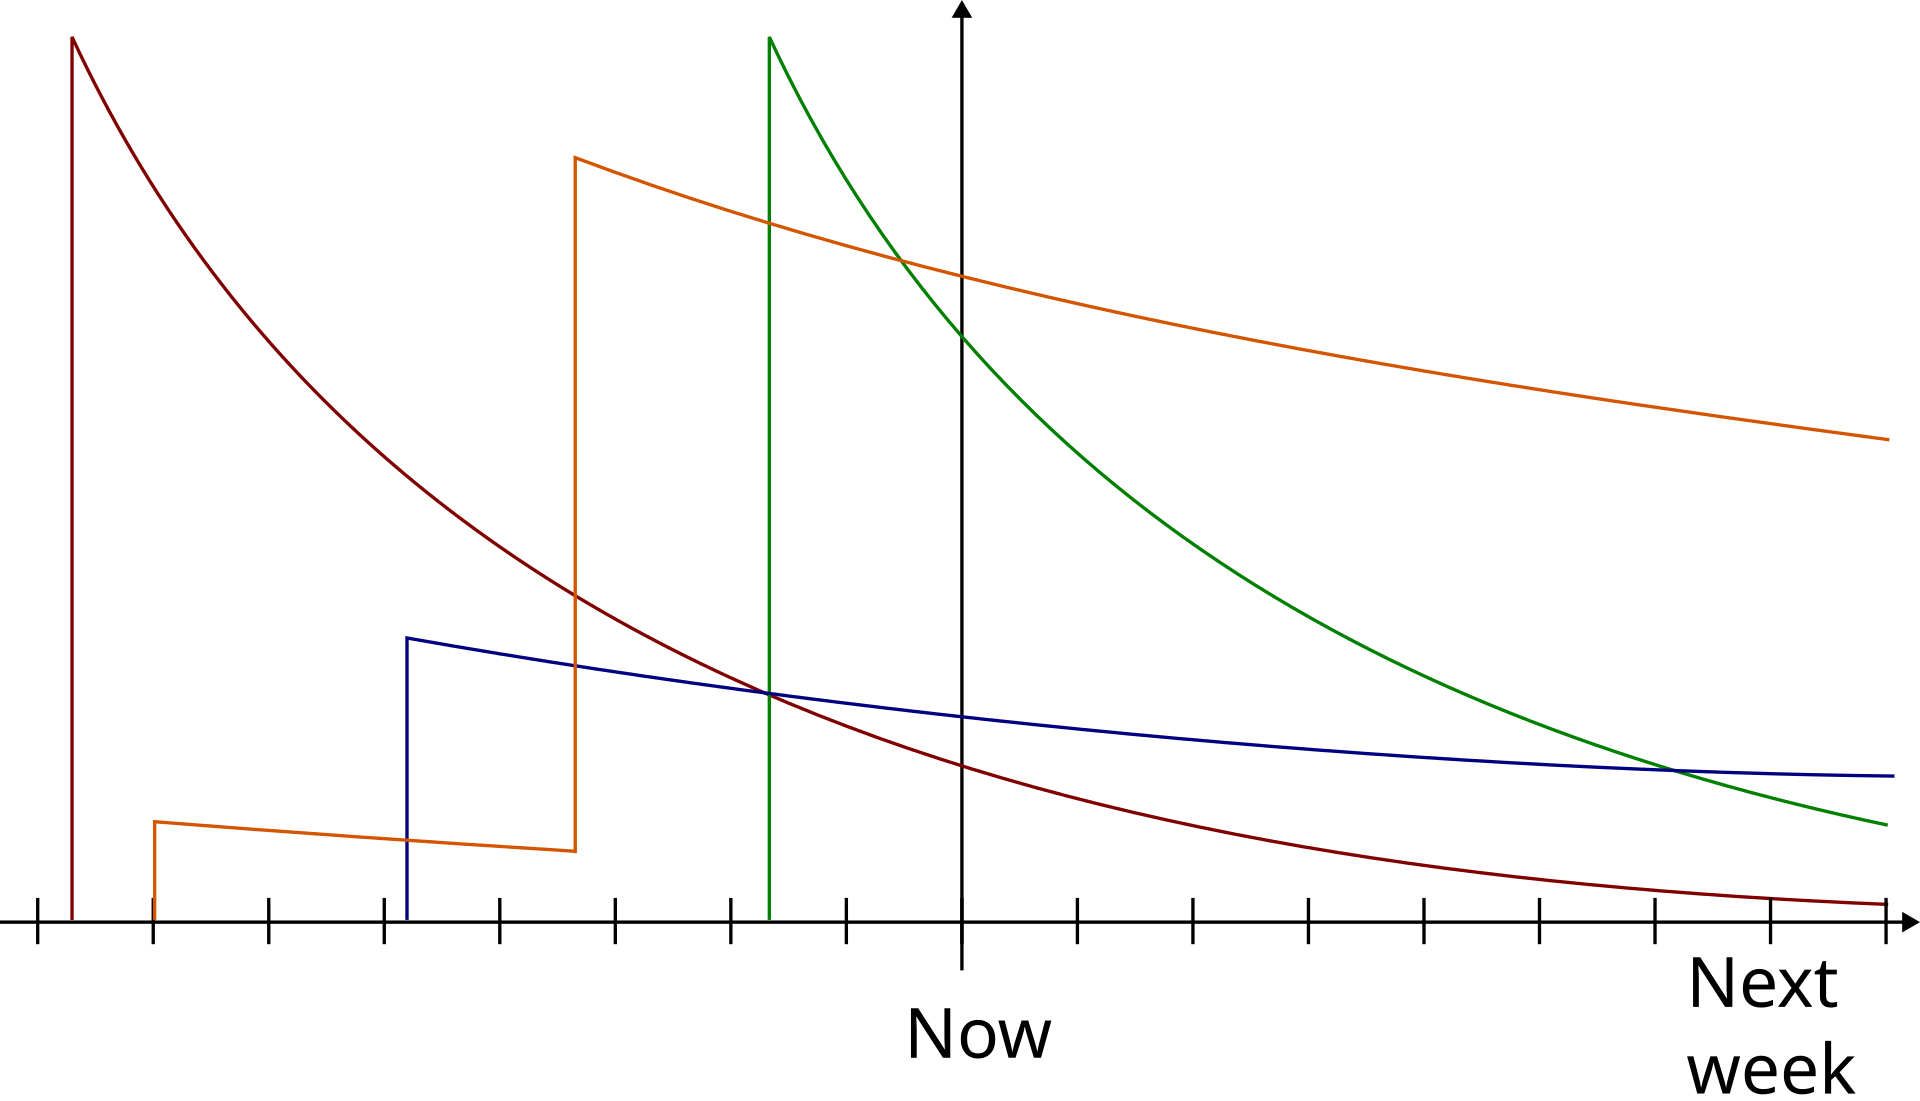
\includegraphics[width=.7\linewidth]{veche_recommender_interface.png}
    \caption{
        Interface for a Veche recommender to visualize their recommendations.
        Each line corresponds to the recommendation of an entity.
        The dark red and dark green lines correspond to a lifetime of 4 days.
        The dark blue corresponds to a lifetime of a month.
        The orange line is a relay, which was then heavily positively evaluated
        for massive recommendations,
        with a lifetime of a month.
        At the present time, the orange entity is the most recommended, 
        ahead of the green, blue and red.
        However, due to diverging lifetimes,
        the blue entity will eventually be more recommended.
    }
    \label{fig:veche-recommender-interface}
\end{figure}

\paragraph{Including additional signals such as ratings and comparisons.}
A user $u \in [U]$ may also want 
to better monitor the ballots $b_u$ sent by their algorithmic representatives,
as presented in Figure~\ref{fig:veche-recommender-interface},
and to modify them based on their own preferences.
This could be done through a better control of the initial values $b_u^0$,
or through comparison interfaces that allows the user to report
that they prefer recommending $e$ over $f$, i.e. they want $b_{ue} (t) \geq b_{uf} (t)$.
Finally, a user's preferences could be generalized to entities they have not evaluated or reposted.
We refer 
to \cite{DBLP:conf/aaai/FageotFHV24,DBLP:journals/corr/abs-2602-08033} 
for ressources on how this could be achieved.
While such approaches may be valuable to allow users $u$ 
to better control their algorithmic representatives,
because of the added complexity they imply,
we keep further considerations out of the scope of this paper.

% \begin{algorithm}
% \caption{User $u$'s generalized algorithmic representative}\label{alg:ballot}
% \begin{algorithmic}
% \Require Post actions $b_{u}^0 \in \setR^E$ at times $t_u \in (\setR \cup \set{\infty})^E$ 
%     with characteristic time $\tau_u \in \setR^E_{>0}$.
% \Require Base characteristic time $\tau_{u0} > 0$, long-term bias $\gamma_u \in \setR$.
% \Require Weights of time scale's own preferred parameters $\lambda_{u \tau}, \lambda_{u\gamma} \in [0, 1]$.
% \Require Intensity of semantic bias $\gamma_u^\measuredangle \geq 0$
% \Require Alice's preferred time parameters $\tau_{Alice} > 0$ and $\gamma_{Alice}$.
% \Require Current time $t \in \setR$.
% \State $\gamma_{u}^{Alice} \gets \lambda_{u \gamma} \gamma_{u} + (1 - \lambda_{u \gamma}) \gamma_{Alice}$ 
%     \Comment{Aggregates $u$ and Alice's preferred short-term bias} \\
% \State $\forall e \in [E] \mathsep 
%     \tau_{ue}^{Alice} \gets \tau_{ue}^{\lambda_{u \tau}} \tau_{Alice}^{1-\lambda_{u \tau}}$ 
%     \Comment{Aggregates $u$ and Alice's preferred time scale} \\
% \State $\forall e \in [E] \mathsep 
%     b_{ue}(t) \gets b_{ue}^0 \frac{
%         \tau_{ue}^{Alice} \ln (1+\tau_{ue}^{Alice}/\tau_{u0})^{\gamma_u^{Alice}}
%     }{(t + \tau_{ue}^{Alice})^2}$ 
%     \Comment{Equals zero for undefined time $t_u = \infty$ (no action)} \\
% \State $\forall e \in [E] \mathsep 
%     b_{ue}^\measuredangle (t) \gets b_{ue} (t) \left(
%         1 + \frac{x_{Alice}^T x}{\norm{x_{Alice}}{2} \cdot \norm{x_e}{2}}
%     \right)^{\gamma_u^\measuredangle}$ 
%     \Comment{Semantic bias} \\
% \State $\forall e \in [E] \mathsep 
%     b_{ue}^\leadsto (t) \gets b_{ue}^\measuredangle (t) 
%         + \sum_{v \in \bU_u^\leadsto} r_{uv} (t) b_{ue}^\leadsto (t)$ 
%     \Comment{Liquid democracy} \\
% \Return $b_u^\leadsto (t) \in \setR^E$
% \end{algorithmic}
% \end{algorithm}

% Algorithm~\ref{alg:ballot} presents the generalized algorithmic representative.
% We stress that the decay function is used by followed users to construct their ballots.
% Alice cannot control the users' ballots.
% Having said this, if she can collect the values of $t_{ue}$ 
% (which are partially public in Tournesol, and fully public in the AT protocol),
% she may use them to reweight the followed users' ballots accordingly to her time preferences.
% Note that all subsequent generalizations will only refer to Alice's ballot aggregation,
% not to the followed users' ballot construction,
% and will thus be under the control of Alice.

% \paragraph{Aggregating all algorithmic representative generalizations.}
% We summarize all the generalizations in the following algorithms.
% In Table~\ref{table:algorithmic_representative_hyperparameters}, 
% we provide values of the hyperparameters which we believe could be reasonable on Tournesol and on BlueSky.


\subsection{Future developments of \Veche{} to improve resilience}
\label{sec:interoperability}

\paragraph{Extended ballots and retrocompatibility.}
By construction, \Veche{} accepts any ballots $b_u \in \setR^E$.
In practice, for communication efficiency,
it may simply collect partial ballots $b_u \in \setR^{<E}$,
where $\setR^{< E} \triangleq \bigcup_{\bE \subset [E]} \setR^\bE$.
The missing coordinates may simply be filled as equal to zero.
In future versions, 
\Veche{} could also accept lifetimes $\tau_u \in \setR^{<E}_{>0}$,
with retrocompatibility defining a default value for unspecified lifetimes
that may typically match the hyperparameter $\tau_0$.
Similarly, as is done in Solidago~\cite{hoang2022solidago},
\Veche{} could additionally accept 
the left and right uncertainties
$\Delta_u^{left}, \Delta_u^{right} \in \setR^{<E}_{\geq 0}$,
with $\Delta_{ue}^{left} = \Delta_{ue}^{right} = 0$ as the default values
for specified ballots $b_{ue}$,
and $\Delta_{ue}^{left} = \Delta_{ue}^{right} = \infty$ 
if $b_{ue}$ was not specified.
Finally, as discussed in~\ref{app:geometric-median},
\Veche{} could consider a hyperparameter $\nu \in \setR^{< E}_{\geq 0}$,
where $\nu_e$ reports the extent to which user $u$ cares about affecting
the weight $w_e$.
Its default value could be $\nu_e = 1$.

\paragraph{Interoperability.}
By construction, \Veche{} is highly interoperable.
Followed user $u \in [U]$ may use any algorithmic representative,
as long as it returns a ballot $b_u \in \setR^E$ 
at any given time $t \in \setR$.
Alice could also leverage generalizations or alternatives to \Veche{},
as long as they leverage similar ballots.
As we will see, practical computational constraints may however restrict
the designs of the algorithmic representatives and ballot aggregations.

\paragraph{Decentralization.}
Alice could host her own \Veche{} server.
At least in principle, 
Veche servers have no need to be hosted on the same machine.
Additionally, in principle,
all followed users $u \in [U]$ 
could have their own algorithmic representative servers.
Upon Alice's request for a new feed,
Alice's \Veche{} server would query ballots 
from the followed users' algorithmic servers.
Once ballots are collected, the \Veche{} server would construct a feed,
which would be sent to Alice.

While this approach highlights the interoperability of \Veche{},
and the sovereignty this may allow,
it may be too slow in practice,
especially if Alice expects an answer within a fraction of a second.
In particular, a dilemma would arise for Alice's \Veche{} server,
between systematically waiting for all ballots to be received,
and halting before all are received,
at the risk of systmatically discriminating 
slow algorithmic representative servers.

To provide better performance guarantees,
followed users may be asked 
to upload their algorithmic representatives 
to Alice's \Veche{} server.
This is where the name \Veche{} takes all its meaning.
Alice's \Veche{} server would thereby be 
an Assembly of algorithmic representatives.
Upon Alice's feed query, the \Veche{} server 
would execute the algorithmic respresentatives' codes,
thereby yielding ballots $b$, 
which the \Veche{} server can turn into a feed.

Computational time constraints still hold however in this setting,
as the \Veche{} is still required to answer within a fraction of a second.
This implies that each algorithmic representative must have a fast running time,
upon query at any point.

\paragraph{Verifiability.}
In practice, Alice will more likely default 
to a \Veche{} server she does not administer,
rather than setting up her own \Veche{} server.
Similarly, followed users may leverage algorithmic representatives
managed by third parties.
To provide Alice with guarantees that her recommendations
were indeed obtained by running \Veche{}
with her followers' algorithmic representatives,
the \Veche{} server could leverage verifiable computing,
and in particular SNARKs,
to prove the correctness of its computations.
Similarly, the \Veche{} server could provide proofs to the followed users
that their algorithmic respresentatives' ballots were correctly accounted for,
and that their algorithmic representatives ran the correct computations
to recommend what the followed users intended to recommend.

\paragraph{Privacy.}
A followed user could prefer to hide their recommendations 
from Alice's \Veche{} server, and perhaps even from Alice.
Typically, the user may want to spread a news,
without Alice knowing the identity of the person 
who wanted the news to be shown to her.
Similarly, Alice could want to hide her feed,
or the list of her followed users, 
from her \Veche{} server.
Providing such privacy guarantees is however a nontrivial open problem,
which we leeave to future work.

\paragraph{Governance.}
We stress that the hyperparameters of the aggregation are under Alice's control.
At least in a setting of algorithmic pluralism where each consumer (like Alice)
is given greater control over the recommendations they receive,
she will be able to tune herself the impact of the different sources of influence.
Having said this, we also stress that, in practice,
most consumers do not engage in algorithmic reconfiguration,
so that the default value chosen for a widely used recommendation system
will heavily influence the dynamics of consumption, production and evaluation 
of the entities that are communicated through the recommendation system.
We believe that an appropriate governance 
for the selection of the default recommendation system is of the utmost importance.

Additionally, as we discuss it in Section~\ref{sec:evaluation},
\Veche{} is likely to generate heavily biased filter bubbles,
as any two consumers' lists of followed users may greatly differ.
To prevent induced polarization risks,
we believe that additional coordinated measures should be considered,
to promote uniting entities of public interest~\cite{hoang2025tournesol}.

Finally, as proposed in~\cite{hoang2022solidago},
the recommendation ecosystem should arguably avoid 
the emergence of \emph{mass influencers},
i.e. users who can massively bias the diffusion of entities,
to prevent the massive spread of a dangerously misleading entity.
This could be done by limiting the cumulative volume of any influencer.
Better yet, as discussed in~\cite{hoang2022solidago},
a \emph{presumption of non-recommendability} could be enforced, 
i.e. an entity would require approval from sufficiently many entities
to obtain the right to be recommended more than 1,000 times per day.
Proposing mechanisms to provide such guarantees is however 
beyond the scope of the paper, 
but represents an exciting future research direction.
